\secspace
\section{Evaluation} 
\label{sec:eval}
In this section, we evaluate \system's ability to protect individual video
frames from style mimicry. \S\ref{sec:setup} describes our video
datasets and experimental setup. \S\ref{sec:eval-metrics} introduces
our metrics for evaluation. \S\ref{sec:protection-robustness}-\ref{sec:video-types}
present results on \system's protection and efficiency. Due to the subjective
nature of interpreting successful style mimicry and visual nature of videos,
we evaluate protection using both automated metrics from existing work, as
well as visual judgement in a user study.

\para{Summary of results.}
Naive perturbations protect videos against style mimicry attempts 64.3\% of
the time according to surveyed users. However, perturbation removal attacks
on naive perturbations successfully recover video style, causing protection
rate to drop to 23.8\% (compared to completely unprotected videos at
17.7\%). \system{} is able to maintain protection even against removal
attacks, restoring protection against style mimicry attempts to 64.5\%. 
We verify that \system~ is able to preserve image perturbations across
consecutive image frames on a diverse set of videos genres and types, and is
robust against our averaging attack introduced in \S\ref{sec:eval-limitations}. 

\subsection{Experimental Setup} 
\label{sec:setup}
\para{Video datasets.}
We evaluate the effectiveness of \system~ on five diverse datasets, covering
different animations, as well as human actions and scenery. On average, each
video contains 6289 total frames. Our experiments conducted on YouTube videos
are for research purposes only, and trained models are deleted at the
conclusion of the study~\cite{fairuse}.
\begin{enumerate}
\item \textbf{Video Games}: 20 randomly selected YouTube videos from a single
  channel showcasing in-game content of different video games, ranging from 2
  to 6 minutes long.
\item \textbf{Human Actions}: 20 randomly selected untrimmed videos of human
  actions from the THUMOS-15 training dataset originally designed for action
  classification~\cite{Idrees_2017}, ranging from 1 to 4 minutes long.
\item \textbf{Japanese Anime}: 20 randomly selected YouTube videos from
  different channels of Japanese animated movies and tv-shows, ranging from 1
  to 5 minutes long.
\item \textbf{Animated Movies}: 10 randomly selected compilations of animated
  (Disney, Pixar, Sony) movie clips, ranging from 5 to 13 minutes long.
\item \textbf{Nature and Wildlife}: 10 randomly selected YouTube videos of
  animals and scenery in the wild, shot in a documentary format. Original
  videos are 30-60 minutes long, we clip each video to the first 2 minutes.
\end{enumerate}

We include three unique animation styles, Video Game (3D
rigs~\cite{videogameanimation}), Japanese Anime (hand
drawn~\cite{animeanimation}), and Animated Movies
(CGI~\cite{amoviesanimation}). The remaining two video datasets are selected
to cover the other types of video imagery, including real human presence
and photography/aerial footage. As a preprocessing step, we maintain
consistent quality among all videos by center cropping videos to square and
resizing to 512x512.  

\para{Defense configuration.}  To showcase the generalizability of \system~
to multiple image-based protection systems, we test \system~ on three such
algorithms: Mist, Anti-DB, and Glaze. We re-implement each defense using
$l_{\infty}$ bounded projected gradient descent (PGD), and use a consistent
targeted image generation method for all three~\cite{shan2023glaze}. As is
standard in image-based PGD methods, we constrain maximum absolute change
in each image pixel to 0.07.

\para{Mimicry configuration.}  We base our style mimicry setup on existing
work~\cite{mist,shan2023glaze,shan2023prompt,antidb} and adapt it to video
frames:
\begin{packed_enumerate}
\item Split each video into partitions using our scene splitting algorithm from \S\ref{sec:method}.
\item Use the CLIP aesthetic model to identify the frame with the highest image quality score within a scene, and select the highest quality images based on scenes with the highest image quality score.
\end{packed_enumerate}
    
We find that all datasets could successfully train style mimicry models with
30 images, except for Animated Movies, which required 60. Here, we can apply the pixel 
averaging adaptive mimicry attack, finetuning on 80\% of extracted images
and saving the remaining 20\% for testing. We use Dreambooth to
finetune a Stable Diffusion 2.1 model on the finetuning dataset for 1000
steps and learning rate of 1e-5. To generate matching synthetic images, we
generate captions from testing images with BLIP~\cite{li2022blip}, and query
the finetuned model to create a set of style mimicked images. 

We evaluate \system~ across several combinations of our proposed defense
system and style mimicry configurations. For each existing perturbation
algorithm, we evaluate the efficacy when perturbed images are untouched, and
when our image averaging attack is used. We evaluate the efficacy of \system~
against style mimicry only when the image averaging attack is used. We also
train a style mimicry model on every video where the frames are left
untouched.

\subsection{Evaluation Metrics}
\label{sec:eval-metrics}
The two key contributions of \system~ are robustness under potential
adversary attack, and reduction in computation costs, which we will evaluate
using the following metrics.

\para{Robustness.}  We measure robustness in two ways. The first two metrics
capture how well image perturbations can withstand adversarial attack. The
last two measure the impact that \system~ has on the quality of images
generated by style mimicry models.
\begin{packed_itemize}
\item \textbf{Latent $L_2$ Norm:} We employ the image encoder used in
  diffusion models to calculate latent representations of perturbed and
  non-perturbed (original) frames, and then calculate the $L_2$ distance
  between them as a measurement for image closeness. For example, a
  successful averaging attack on consecutively perturbed frames would lead to
  low latent $L_2$ norm, while a robust system should maintain a high latent
  $L_2$ norm. In particular, this metric isolates how diffusion models
  capture image differences. 
\item \textbf{Mean Pixel Difference:} We also measure the differences between
  images at a pixel level, motivated by the $l_{\infty}$ bounded pixel
  changes that all three of our defense algorithms are constrained by. Mean
  Pixel Difference (MPD) is model-agnostic, and defined as the average of all
  pixel differences between a perturbed image and original image. Similar to
  the latent $L_2$ norm, a higher MPD between perturbed and original frames
  signals higher protection.
\item \textbf{CLIP-Genre Shift:} We adapt a metric used in existing
  work~\cite{shan2023glaze} to demonstrate the effectiveness
  of \system~ at disrupting style mimicry. Intuitively, existing image
  perturbation algorithms are designed to cause diffusion models to learn the
  wrong artistic style. Thus, we can measure the success of \system's
  protection by calculating the percentage of generated images in which a
  CLIP image classifier unsuccessfully predicts the ground-truth style from
  training images. A higher CLIP-based Genre Shift score equates to stronger
  protection, while the opposite equates to stronger style mimicry. However, it 
  is a granular metric and its correlation to visual properties might be weak.
\item \textbf{Human-rated protection success rate (PSR):} To accurately capture 
  end-to-end visual properties, we perform
  two IRB-approved user studies (more details on participants in
  Appendix~\ref{app:detailed-user-study}) where participants look at images
  generated by 
  mimicry models and rate if the style mimicry was successful. The first asks
  artist volunteers to 
  rate performance on our two ``Art'' datasets: Anime and Video Games. The
  second asks general users to rate performance on all 5 datasets. For
  each video, we train 10 style mimicry models, matching our experiment
  configuration. For each mimicry model, we show participants 5 frames from
  the original video next to 5 frames generated by the mimicry model. Each
  participant is shown one example from each experiment configuration,
  randomly selected from the set of 80 videos (3 datasets x 20 videos + 2
  datasets x 10 videos each).

  \indent We ask participants to compare original
  video frames to those generated by mimicry, and rate the success on a 5-point
  Likert scale (ranging from ``Not successful at all'' to ``Very
  successful''). Following prior work, we define protection success rate as
  the percent of participants who rated how well generated images mimic
  original style as ``Not very well'' or ``Not well at all.'' We also show
  artists short 10 second clips of videos glazed naively and with
  \system. Here, we ask how noticeable the perturbations are on a 5 point
  Likert scale ranging from ``Very noticeable'' to ``Not noticeable at all.''
  We define \textit{Noticeability Rate} (NR) as the \% of users that think
  perturbations are ``Noticeable'' or ``Very noticeable.''
\end{packed_itemize}

\para{Computation efficiency:} 
Finally, we also measure the computation speed of \system. Here, we only experiment on one image perturbation algorithm due to computational constraints. Glaze is chosen due to its balance of speed (fastest of the three) and strong robustness. For each video, we conduct our measurement on a single A100 GPU.
\begin{packed_itemize}
\item \textbf{Speedup Factor:} We compute speedup factor as time taken to apply (naive)
  protection to every frame, divided by time taken to protect the video using
  \system.  Because of the compute time involved, we estimate full (naive) protection by estimating per frame protection time, scaled up by number of frames in the video.
\item \textbf{Seconds per Frame:} We also report the average time it takes to
  perturb each frame in a video. This provides a grounding metric that is not
  relative like speedup factor.
\end{packed_itemize}

\begin{table*}[t]
    \centering
    \resizebox{0.88\textwidth}{!}{
      \begin{tabular}{cccccccccc}
        & \multicolumn{3}{c}{Glaze}                                                                                                                                               & \multicolumn{3}{c}{Mist}                                                                                                                                                & \multicolumn{3}{c}{Anti-DB}                                                                                                                        \\ \cline{2-10} 
        & Naive              & \begin{tabular}[c]{@{}c@{}}Naive\\ + Attack\end{tabular} & \multicolumn{1}{c|}{\textbf{\begin{tabular}[c]{@{}c@{}}\system\\ + Attack\end{tabular}}} & Naive              & \begin{tabular}[c]{@{}c@{}}Naive\\ + Attack\end{tabular} & \multicolumn{1}{c|}{\textbf{\begin{tabular}[c]{@{}c@{}}\system\\ + Attack\end{tabular}}} & Naive              & \begin{tabular}[c]{@{}c@{}}Naive\\ + Attack\end{tabular} & \textbf{\begin{tabular}[c]{@{}c@{}}\system\\ + Attack\end{tabular}} \\ \hline
\multicolumn{1}{c|}{Video Game}          & 406.69 $\pm$ 20.09 & 262.82 $\pm$ 32.39                                       & \multicolumn{1}{c|}{425.19 $\pm$ 26.84}                                                 & 468.51 $\pm$ 40.68 & 296.29 $\pm$ 38.53                                       & \multicolumn{1}{c|}{496.04 $\pm$ 43.52}                                                 & 400.48 $\pm$ 35.12 & 240.38 $\pm$ 37.83                                       & 421.66 $\pm$ 37.01                                                 \\
\multicolumn{1}{c|}{Japanese Anime}      & 395.86 $\pm$ 20.32 & 284.51 $\pm$ 53.59                                       & \multicolumn{1}{c|}{406.93 $\pm$ 26.87}                                                 & 467.00 $\pm$ 43.44 & 319.77 $\pm$ 56.92                                       & \multicolumn{1}{c|}{493.53 $\pm$ 47.91}                                                 & 406.04 $\pm$ 41.29 & 272.34 $\pm$ 59.09                                       & 424.51 $\pm$ 41.96                                                 \\
\multicolumn{1}{c|}{Animated Movies}     & 380.04 $\pm$ 17.52 & 308.06 $\pm$ 47.66                                       & \multicolumn{1}{c|}{406.30 $\pm$ 26.05}                                                 & 475.07 $\pm$ 39.40 & 349.04 $\pm$ 51.88                                       & \multicolumn{1}{c|}{496.81 $\pm$ 42.17}                                                 & 404.55 $\pm$ 37.85 & 299.84 $\pm$ 55.27                                       & 422.11 $\pm$ 38.46                                                 \\
\multicolumn{1}{c|}{Nature and Wildlife} & 402.10 $\pm$ 17.24 & 319.23 $\pm$ 53.86                                       & \multicolumn{1}{c|}{408.62 $\pm$ 25.91}                                                 & 466.05 $\pm$ 41.64 & 346.28 $\pm$ 56.05                                       & \multicolumn{1}{c|}{496.48 $\pm$ 41.38}                                                 & 393.73 $\pm$ 30.02 & 297.58 $\pm$ 58.51                                       & 412.73 $\pm$ 30.82                                                 \\
\multicolumn{1}{c|}{Human Actions}       & 370.77 $\pm$ 27.41 & 316.53 $\pm$ 50.39                                       & \multicolumn{1}{c|}{397.97 $\pm$ 27.03}                                                 & 494.19 $\pm$ 39.40 & 369.70 $\pm$ 48.57                                       & \multicolumn{1}{c|}{508.08 $\pm$ 39.06}                                                 & 415.92 $\pm$ 36.58 & 316.19 $\pm$ 50.97                                       & 426.26 $\pm$ 35.29                                                
\end{tabular}
    }
    \caption{Latent $L_2$ norm between original and perturbed frames across all datasets and image perturbation algorithms. Averaging attack reduces perturbation effectiveness from naive video cloaking (attacked naive $<<$ naive), but is unsuccessful against \system~.}
    \label{tab:adv-algorithm-robustness-loss}
\end{table*}

\begin{table*}[t]
    \centering
    \resizebox{0.88\textwidth}{!}{
      \begin{tabular}{cccccccccc}
        & \multicolumn{3}{c}{Glaze}                                                                                                                                               & \multicolumn{3}{c}{Mist}                                                                                                                                                & \multicolumn{3}{c}{Anti-DB}                                                                                                                        \\ \cline{2-10} 
        & Naive              & \begin{tabular}[c]{@{}c@{}}Naive\\ + Attack\end{tabular} & \multicolumn{1}{c|}{\textbf{\begin{tabular}[c]{@{}c@{}}\system\\ + Attack\end{tabular}}} & Naive              & \begin{tabular}[c]{@{}c@{}}Naive\\ + Attack\end{tabular} & \multicolumn{1}{c|}{\textbf{\begin{tabular}[c]{@{}c@{}}\system\\ + Attack\end{tabular}}} & Naive              & \begin{tabular}[c]{@{}c@{}}Naive\\ + Attack\end{tabular} & \textbf{\begin{tabular}[c]{@{}c@{}}\system\\ + Attack\end{tabular}} \\ \hline
\multicolumn{1}{c|}{Video Game}          & 111.99 $\pm$ 11.50 & 85.00 $\pm$ 12.37                                        & \multicolumn{1}{c|}{108.54 $\pm$ 12.66}                                                 & 120.88 $\pm$ 6.79  & 102.91 $\pm$ 14.20                                       & \multicolumn{1}{c|}{119.26 $\pm$ 7.52}                                                  & 124.64 $\pm$ 5.94  & 98.21 $\pm$ 14.69                                        & 121.10 $\pm$ 7.49                                                  \\
\multicolumn{1}{c|}{Japanese Anime}      & 112.31 $\pm$ 12.92 & 91.03 $\pm$ 14.44                                        & \multicolumn{1}{c|}{108.25 $\pm$ 14.26}                                                 & 120.84 $\pm$ 8.71  & 106.25 $\pm$ 15.08                                       & \multicolumn{1}{c|}{119.03 $\pm$ 9.88}                                                  & 124.34 $\pm$ 7.94  & 103.01 $\pm$ 15.91                                       & 120.27 $\pm$ 10.27                                                 \\
\multicolumn{1}{c|}{Animated Movies}     & 109.43 $\pm$ 13.14 & 89.92 $\pm$ 12.16                                        & \multicolumn{1}{c|}{107.57 $\pm$ 13.56}                                                 & 122.22 $\pm$ 8.59  & 109.44 $\pm$ 15.08                                       & \multicolumn{1}{c|}{121.37 $\pm$ 9.19}                                                  & 125.89 $\pm$ 7.98  & 106.27 $\pm$ 15.99                                       & 122.42 $\pm$ 9.21                                                  \\
\multicolumn{1}{c|}{Nature and Wildlife} & 115.14 $\pm$ 5.39  & 98.65 $\pm$ 12.56                                        & \multicolumn{1}{c|}{109.96 $\pm$ 8.23}                                                  & 121.54 $\pm$ 3.13  & 110.49 $\pm$ 10.65                                       & \multicolumn{1}{c|}{120.80 $\pm$ 4.81}                                                  & 124.79 $\pm$ 2.30  & 108.15 $\pm$ 13.53                                       & 120.92 $\pm$ 5.25                                                  \\
\multicolumn{1}{c|}{Human Actions}       & 109.61 $\pm$ 16.02 & 90.18 $\pm$ 15.91                                        & \multicolumn{1}{c|}{108.22 $\pm$ 16.41}                                                 & 120.85 $\pm$ 14.49 & 108.19 $\pm$ 21.66                                       & \multicolumn{1}{c|}{119.06 $\pm$ 16.02}                                                 & 124.52 $\pm$ 14.13 & 105.51 $\pm$ 23.66                                       & 120.09 $\pm$ 16.64                                                
\end{tabular}
    }
    \caption{Mean pixel difference (MPD) between original and perturbed frames across all datasets and image perturbation algorithms. Averaging attack reduces perturbation effectiveness from naive video cloaking (attacked naive $<<$ naive), but is unsuccessful against \system~.}
    \label{tab:adv-algorithm-robustness-pd}
\end{table*}


\begin{table*}[t]
    \centering
    \resizebox{0.88\textwidth}{!}{
      \begin{tabular}{cccccccccccc}
        \multirow{2}{*}{}                                                        & \multirow{2}{*}{}                         &                                       & \multicolumn{3}{c}{Glaze}                                                                                                                                             & \multicolumn{3}{c}{Mist}                                                                                                                                              & \multicolumn{3}{c}{Anti-DB}                                                                                                                      \\ \cline{3-12} 
                                                                                 &                                           & \multicolumn{1}{c|}{Clean}            & Naive            & \begin{tabular}[c]{@{}c@{}}Naive\\ + Attack\end{tabular} & \multicolumn{1}{c|}{\textbf{\begin{tabular}[c]{@{}c@{}}\system\\ + Attack\end{tabular}}} & Naive            & \begin{tabular}[c]{@{}c@{}}Naive\\ + Attack\end{tabular} & \multicolumn{1}{c|}{\textbf{\begin{tabular}[c]{@{}c@{}}\system\\ + Attack\end{tabular}}} & Naive            & \begin{tabular}[c]{@{}c@{}}Naive\\ + Attack\end{tabular} & \textbf{\begin{tabular}[c]{@{}c@{}}\system\\ + Attack\end{tabular}} \\ \hline
        \multirow{2}{*}{Artist}                                                  & \multicolumn{1}{c|}{Video Game}           & \multicolumn{1}{c|}{15.05 $\pm$ 1.10} & 92.23 $\pm$ 0.72 & 19.35 $\pm$ 1.13                                         & \multicolumn{1}{c|}{97.98 $\pm$ 0.52}                                                   & 82.88 $\pm$ 0.85 & 14.81 $\pm$ 1.08                                         & \multicolumn{1}{c|}{91.01 $\pm$ 0.69}                                                   & 93.26 $\pm$ 0.69 & 23.71 $\pm$ 1.25                                         & 91.74 $\pm$ 0.67                                                   \\
                                                                                 & \multicolumn{1}{c|}{Japanese Anime}       & \multicolumn{1}{c|}{24.27 $\pm$ 1.13} & 82.88 $\pm$ 0.97 & 27.03 $\pm$ 1.13                                         & \multicolumn{1}{c|}{72.32 $\pm$ 1.00}                                                   & 68.69 $\pm$ 0.97 & 34.74 $\pm$ 1.18                                         & \multicolumn{1}{c|}{65.77 $\pm$ 1.10}                                                   & 79.44 $\pm$ 0.83 & 36.19 $\pm$ 1.14                                         & 83.84 $\pm$ 0.83                                                   \\ \hline
        \multirow{5}{*}{\begin{tabular}[c]{@{}c@{}}General\\ Users\end{tabular}} & \multicolumn{1}{c|}{Video Game}           & \multicolumn{1}{c|}{20.14 $\pm$ 1.13} & 85.59 $\pm$ 0.82 & 18.26 $\pm$ 1.11                                         & \multicolumn{1}{c|}{88.99 $\pm$ 0.76}                                                   & 86.84 $\pm$ 0.87 & 16.67 $\pm$ 1.06                                         & \multicolumn{1}{c|}{95.24 $\pm$ 0.65}                                                   & 73.87 $\pm$ 1.02 & 25.20 $\pm$ 1.17                                         & 80.39 $\pm$ 0.97                                                   \\
                                                                                 & \multicolumn{1}{c|}{Japanese Anime}       & \multicolumn{1}{c|}{20.95 $\pm$ 1.07} & 66.07 $\pm$ 1.05 & 21.21 $\pm$ 1.09                                         & \multicolumn{1}{c|}{54.63 $\pm$ 1.07}                                                   & 59.46 $\pm$ 1.18 & 26.50 $\pm$ 1.14                                         & \multicolumn{1}{c|}{68.80 $\pm$ 1.03}                                                   & 49.00 $\pm$ 1.07 & 19.61 $\pm$ 0.99                                         & 52.53 $\pm$ 1.21                                                   \\
                                                                                 & \multicolumn{1}{c|}{Animated Movies}      & \multicolumn{1}{c|}{14.81 $\pm$ 1.19} & 44.83 $\pm$ 1.15 & 14.81 $\pm$ 1.04                                         & \multicolumn{1}{c|}{36.51 $\pm$ 1.16}                                                   & 35.00 $\pm$ 1.04 & 16.67 $\pm$ 1.06                                         & \multicolumn{1}{c|}{50.91 $\pm$ 1.19}                                                   & 26.79 $\pm$ 1.14 & 12.24 $\pm$ 1.03                                         & 35.94 $\pm$ 1.12                                                   \\
                                                                                 & \multicolumn{1}{c|}{Nature and Wildlife}  & \multicolumn{1}{c|}{8.89 $\pm$ 1.02}  & 78.43 $\pm$ 0.80 & 18.06 $\pm$ 1.10                                         & \multicolumn{1}{c|}{65.38 $\pm$ 1.02}                                                   & 68.63 $\pm$ 0.98 & 20.41 $\pm$ 1.07                                         & \multicolumn{1}{c|}{85.00 $\pm$ 0.73}                                                   & 69.49 $\pm$ 1.16 & 31.34 $\pm$ 1.34                                         & 64.15 $\pm$ 1.01                                                   \\
                                                                                 & \multicolumn{1}{c|}{Generic Video Scenes} & \multicolumn{1}{c|}{15.05 $\pm$ 1.03} & 70.64 $\pm$ 1.05 & 42.42 $\pm$ 1.18                                         & \multicolumn{1}{c|}{49.02 $\pm$ 1.17}                                                   & 54.00 $\pm$ 1.05 & 38.74 $\pm$ 1.15                                         & \multicolumn{1}{c|}{60.00 $\pm$ 1.06}                                                   & 62.73 $\pm$ 1.15 & 21.51 $\pm$ 1.19                                         & 61.21 $\pm$ 1.20                                                  
        \end{tabular}
    }
    \caption{Percentage of \textit{artists} and \textit{general users} who
      deem protection is successful on different videos. Artists rated
      more art-driven videos (Video Games and Japanese Anime), while general
      users rated all videos. Column include naive protection,
      pixel-averaging on naive protection, and pixel-averaging on
      \system{}. Pixel-averaging breaks protection; \system{} restores it.}
    \label{tab:adv-algorithm-robustness-artist}
\end{table*}

\begin{table*}[t]
    \centering
    \resizebox{0.88\textwidth}{!}{
      \begin{tabular}{ccccccccccc}
        &                                      & \multicolumn{3}{c}{Glaze}                                                                                                                                            & \multicolumn{3}{c}{Mist}                                                                                                                                             & \multicolumn{3}{c}{Anti-DB}                                                                                                                     \\ \cline{2-11} 
        & \multicolumn{1}{c|}{Clean}           & Naive           & \begin{tabular}[c]{@{}c@{}}Naive\\ + Attack\end{tabular} & \multicolumn{1}{c|}{\textbf{\begin{tabular}[c]{@{}c@{}}\system\\ + Attack\end{tabular}}} & Naive           & \begin{tabular}[c]{@{}c@{}}Naive\\ + Attack\end{tabular} & \multicolumn{1}{c|}{\textbf{\begin{tabular}[c]{@{}c@{}}\system\\ + Attack\end{tabular}}} & Naive           & \begin{tabular}[c]{@{}c@{}}Naive\\ + Attack\end{tabular} & \textbf{\begin{tabular}[c]{@{}c@{}}\system\\ + Attack\end{tabular}} \\ \hline
\multicolumn{1}{c|}{Video Games}         & \multicolumn{1}{c|}{0.49 $\pm$ 0.23} & 0.85 $\pm$ 0.23 & 0.71 $\pm$ 0.26                                          & \multicolumn{1}{c|}{0.97 $\pm$ 0.07}                                                    & 0.85 $\pm$ 0.20 & 0.75 $\pm$ 0.22                                          & \multicolumn{1}{c|}{0.97 $\pm$ 0.06}                                                    & 0.77 $\pm$ 0.26 & 0.61 $\pm$ 0.26                                          & 0.94 $\pm$ 0.13                                                    \\
\multicolumn{1}{c|}{Japanese Anime}      & \multicolumn{1}{c|}{0.25 $\pm$ 0.18} & 0.76 $\pm$ 0.23 & 0.58 $\pm$ 0.19                                          & \multicolumn{1}{c|}{0.88 $\pm$ 0.13}                                                    & 0.77 $\pm$ 0.24 & 0.60 $\pm$ 0.21                                          & \multicolumn{1}{c|}{0.92 $\pm$ 0.11}                                                    & 0.64 $\pm$ 0.30 & 0.41 $\pm$ 0.23                                          & 0.86 $\pm$ 0.13                                                    \\
\multicolumn{1}{c|}{Animated Movies}     & \multicolumn{1}{c|}{0.45 $\pm$ 0.22} & 0.65 $\pm$ 0.29 & 0.52 $\pm$ 0.28                                          & \multicolumn{1}{c|}{0.68 $\pm$ 0.25}                                                    & 0.61 $\pm$ 0.28 & 0.53 $\pm$ 0.30                                          & \multicolumn{1}{c|}{0.73 $\pm$ 0.21}                                                    & 0.58 $\pm$ 0.31 & 0.46 $\pm$ 0.29                                          & 0.65 $\pm$ 0.28                                                    \\
\multicolumn{1}{c|}{Nature and Wildlife} & \multicolumn{1}{c|}{0.32 $\pm$ 0.15} & 0.80 $\pm$ 0.24 & 0.61 $\pm$ 0.20                                          & \multicolumn{1}{c|}{0.91 $\pm$ 0.12}                                                    & 0.82 $\pm$ 0.18 & 0.53 $\pm$ 0.30                                          & \multicolumn{1}{c|}{0.98 $\pm$ 0.02}                                                    & 0.69 $\pm$ 0.32 & 0.41 $\pm$ 0.22                                          & 0.94 $\pm$ 0.09                                                    \\
\multicolumn{1}{c|}{Human Actions}       & \multicolumn{1}{c|}{0.22 $\pm$ 0.23} & 0.70 $\pm$ 0.32 & 0.50 $\pm$ 0.31                                          & \multicolumn{1}{c|}{0.78 $\pm$ 0.22}                                                    & 0.80 $\pm$ 0.25 & 0.66 $\pm$ 0.27                                          & \multicolumn{1}{c|}{0.94 $\pm$ 0.07}                                                    & 0.68 $\pm$ 0.33 & 0.45 $\pm$ 0.27                                          & 0.81 $\pm$ 0.24                                                   
\end{tabular}
  }
  \caption{CLIP-Genre Shift across all datasets and image perturbation algorithms. Averaging attack decreases the number of images generated of a different style to the original video (attacked naive $\approx$ clean), but fails to do the same against \system~.}
    \label{table:adv-algorithm-style-mimicry}
\end{table*}

\subsection{Robustness against Pixel-Averaging Mimicry}
\label{sec:protection-robustness}
\para{\system~ prevents style mimicry. } 
We showed in \S\ref{sec:eval-limitations} that pixel-averaging attacks can
remove image protection by smoothing them out across similar
frames. We begin by looking at the ability of pixel-averaging methods to extract
frames similar to the original, as measured by pixel level metrics in
Table~\ref{tab:adv-algorithm-robustness-loss} and
\ref{tab:adv-algorithm-robustness-pd}.

For all protection tools, across each category of videos, we see that the
pixel-averaging attack significantly reduces the distance between the
protected frames compared to the originals, measured by both latent $L_2$ norm and
MPD. More importantly, we see that that same pixel-averaging attack fail when
applied to frames protected by \system{}, and it actually increases the
distances from the original.

Next, we turn our attention to the ability of adaptive mimicry attacks and
their ability to produce accurate end-to-end mimicry models. Table~\ref{tab:adv-algorithm-robustness-artist} shows the results of our
two user studies, involving both a population of artists and general users
(participant details in Appendix~\ref{app:detailed-user-study}). While
artists' views varied somewhat from general users across categories, all
users consistently provided the same feedback, that pixel-averaging broke the
protection provided by naive anti-mimicry tools, but \system{} restored that
protection (and in many cases increased protection higher than naive
protection levels). Table~\ref{table:adv-algorithm-style-mimicry} quantified
the same issue of end to end protection, but using the CLIP
CLIP-Genre shift metric. Results are very consistent with those from user
studies. \system{} restored protection broken by pixel-averaging attack and
in many cases, improved protection beyond the original naive levels.

Finally, Figure~\ref{fig:core-style-mimicry-results} shows some examples of
images generated by style mimicry models under our experiment configurations.

\begin{figure}[t]
    \centering
    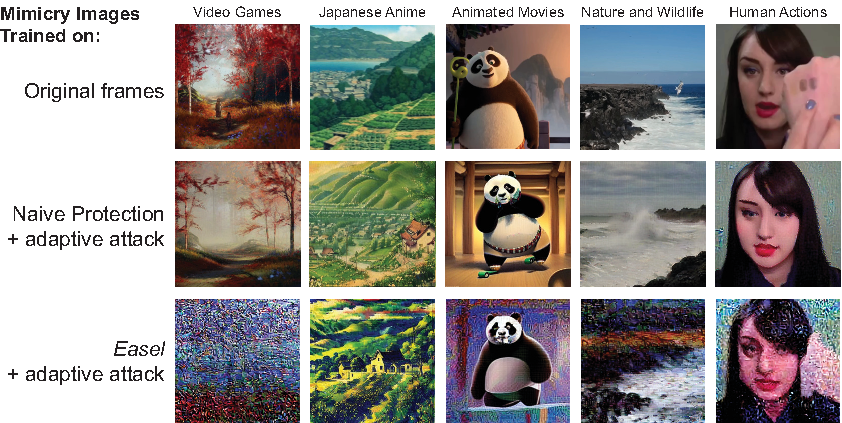
\includegraphics[width=0.95\columnwidth]{plots/core-style-mimicry-results-eps-converted-to.pdf}
    \vspace{-0.1in}
    \caption{Some visual examples of style mimicry on \system~ showing it is
      robust to pixel averaging attack.}
    \label{fig:core-style-mimicry-results}
    \vspace{-0.1in}    
  \end{figure}
\begin{figure}[t]
    \centering
    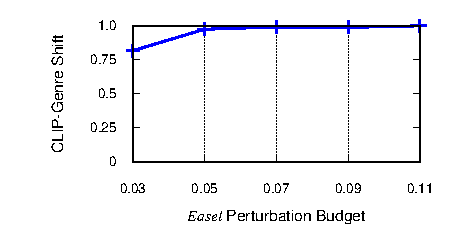
\includegraphics[width=3in]{plots/eval/eps-robustness-eps-converted-to.pdf}
    \vspace{-0.2in}
    \caption{Average robustness (CLIP-Genre Shift) increases as $l_{\infty}$
      perturbation budget increases on 4 Video Game videos. For comparison,
      mimicry on original frames produces CLIP-Genre Shift of 0.44.}
    \label{fig:eps-robustness}
\end{figure}

\para{Impact of perturbation budget on robustness.} 
In Figure~\ref{fig:eps-robustness}, we show that robustness under \system{}
increases with perturbation budget, quickly maxing out after 0.05. This
follows the same trend we see in existing image-only perturbation algorithms. 


\subsection{Computational Costs and Video Quality}
\label{subsec:protection-usability}
In \S\ref{subsec:limitations}, we identified two additional limitations
of a naive application of anti-mimicry tools: high computation overhead and
poor video quality (randomness across per-frame perturbations appear as
flickering snow when viewed at regular speeds). Here, we show that
\system~ significantly improves on both the computation overhead of
perturbing video frames, and increases video quality over naively protected
videos.

\para{\system~ reduces computation overhead. } 
We measure the computation efficiency of \system~ on three of our
datasets. As shown in Table~\ref{tab:adv-algorithm-efficiency}, the Video
Game and Human Actions datasets achieve 7-8x speedup factor when using \system~ over
its naive video protection, while the Japanese Anime dataset achieves just over
4x speedup factor. \system~ would improve computation efficiency of a 5 minute 30
fps video from 88 to 11 hours. This magnitude of speedup factor greatly improves the
usability of applying image-based perturbations to videos, and makes video
protection more reasonable for video creators, particularly smaller or
independent creator groups.

The speedup factor is lowest for Japanese anime videos, likely due to the high movement 
across frames. In practice, we can further improve the speedup by changing our
system parameters, \eg changing second threshold $\tau_2$
from 0.45 to 0.8, which increases speedup factor of the four slowest Japanese Anime videos from 2.12 to 3.90 with a small tradeoff in robustness (more details
in Appendix~\ref{app:num-images-average} and \ref{app:eps-robustness}).  

\begin{table}[t]
    \centering
    \resizebox{0.4\textwidth}{!}{
        \begin{tabular}{c|cc}
            & Avg. Speedup Factor    & Avg. Seconds per Frame \\ \hline
            Video Game     & 7.87 $\pm$ 2.81 & 5.16 $\pm$ 2.13        \\
            Japanese Anime & 4.16 $\pm$ 3.19 & 11.25 $\pm$ 4.55       \\
            Human Action   & 7.37 $\pm$ 4.34 & 7.84 $\pm$ 6.43       
        \end{tabular}
    }
    \caption{\system~ with Glaze enables significant computation speedup factor
      across all Video Game, Japanese Anime, and Human action videos when
      compared to naive video protection. For comparison, naive video
      protection takes on average 35 seconds per frame on a single A100 GPU.}
    \label{tab:adv-algorithm-efficiency}
\end{table}


\begin{table}[t]
    \centering
    \resizebox{0.4\textwidth}{!}{
        \begin{tabular}{c|cc}
            & \multicolumn{2}{c}{\% of Users Notice Perturbations} \\
            & Naive Glaze               & \system~ w/ Glaze           \\ \hline
            Video Game     & 70.30 $\pm$ 1.03          & 21.29 $\pm$ 1.06         \\
            Japanese Anime & 48.73 $\pm$ 1.16          & 18.27 $\pm$ 1.0         
        \end{tabular}
    }
    \caption{Our user study shows that the percentage of users who notice
      perturbations generated by \system~ is
      significantly less than those who notice perturbations in naive video
      protection. (Tests implemented using Glaze).} 
    \label{tab:adv-algorithm-style-mimicry-visual}
\end{table}

\para{\system~ is less visually disruptive/noticeable. }  Even though
image-based perturbation methods are designed to be imperceptible, applying
them naively to videos leads to protected videos that flicker and are
noticeably grainy. This is a result of perturbation masks changing
drastically from frame to frame, a problem that \system~ addresses
directly. In our user study, we show participants 10-second clips of
protected videos from our three datasets. The first video is naively protected
using our implementation of Glaze, and the second video is protected with 
\system{}. Participants are asked to identify how visible the
perturbations are in both 
videos. Table~\ref{tab:adv-algorithm-style-mimicry-visual} presents
\textit{noticeability rate}, showing artists are able to notice perturbations
significantly more when videos are protected naively (70\%) than with
\system~ (21\%).

\begin{table}[t]
    \centering
    \resizebox{0.3\textwidth}{!}{
        \begin{tabular}{c|cc}
            & CLIP-Genre Shift & Speedup Factor          \\ \hline
            15fps & 0.97 $\pm$ 0.04  & 6.11 $\pm$ 1.90  \\
            30fps & 0.98 $\pm$ 0.02  & 9.57 $\pm$ 2.47  \\
            60fps & 1.00 $\pm$ 0.00  & 15.96 $\pm$ 4.06
        \end{tabular}
    }
    \caption{Different framerates do not impact protection
      robustness (CLIP-Genre Shift), but higher framerates lead to higher
      speedup factor under \system. (4 Video Game videos.)} 
    \label{table:fps-test}
\end{table}

\begin{figure}[t]
  \centering
  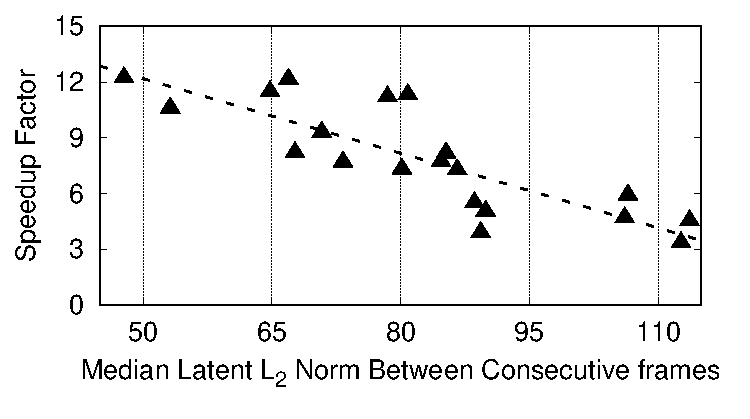
\includegraphics[width=0.9\columnwidth]{plots/eval/consecutive-frames-speedup-eps-converted-to.pdf}
  \vspace{-0.25in}
  \caption{Speedup factor decreases as movement increases between frames (latent $L_2$
    norm) on all Video Game videos.}
  \label{fig:action-across-datasets}
\end{figure}


\subsection{Impact of Video Types on Robustness and Efficiency}
\label{sec:video-types}
Beyond examining the efficacy of \system~ on a variety of video genres, we
also examine four aspects of videos creation/distribution irrespective to
genre that real-world content creators are likely to deal with while posting
videos online. We investigate the effects that framerate, movement between
frames, duration of scenes, and compression, have on robustness and
computation efficiency. We anticipate these as questions that video content
creators are likely to ask with respect to the efficacy of \system. In this
section, we show that \system's robustness holds steady across video types,
while computational efficiency is the most prone to change. 


\para{FPS}
Here, we evaluate the change in robustness and computation efficiency of
\system~ when videos are encoded with a different number of frames per second
(fps). We evaluate \system~ with Glaze on three different framerates, 15fps,
30fps, and 60fps, and measure its performance on four videos from the Video
Game Dataset. 30fps and 60fps are widely used in the video
community~\cite{ytvideosettings}, and we also include 15 to show the effects
that much a slower framerate has on robustness and computation
efficiency. Our results can be found in Table~\ref{table:fps-test}, which
show that framerate does not have significant impact on robustness, but that
increasing framerate from 15fps to 60fps increases speedup factor from 6x to
16x. Thus, we show that \system's computation performance is at its worst
with low framerate, but scales well when content creators choose to increase
framerate in their videos. 


\para{Action within scenes}
Movement within videos is difficult to capture, but we use latent $L_2$ norm between
two image latent representations as a good approximation. Intuitively, minor
movement between frames should lead to minor changes in image latent
representation. In this section, we investigate the effect that latent $L_2$
norm between consecutive frames in video scenes has on computation
efficiency. We measure the latent $L_2$ norm between consecutive frames in a
scene for every video in the Video Game dataset, and compare the median of
the latent $L_2$ norm across scenes to the speedup factor \system~ with Glaze
provides. In Figure~\ref{fig:action-across-datasets}, we show that there is a
negative linear correlation between $L_2$ latent norm and
speedup factor. Intuitively, videos with higher action within scenes are more likely
to require additional optimization in order to better align image
perturbations across fast changing frames. 

Finally, we also analyze the impact of {\bf scene duration} (number of frames per
scene) and {\bf video compression} factor (bitrate of video) on robustness and
speedup factor. We found that these factors have no observable impact.


